%*****************************************
\chapter{ \textbf{Appendix} }\label{ch:Appendix}
%*****************************************
\vspace{0.5cm} 

\section{SQL-queries}\label{sec:SQL}
\lstset{language = SQL}

In this section, the queries performed in the \textit{Gaia} database are shown for the three different fields of Sco-Cen OB Association namely Lower Centaurus Crux (LCC), Upper Centaurus Lupus (UCL), and Upper Scorpius (US).\\    

\textbf{Lower Centaurus Crux (LCC)}
\begin{lstlisting}[frame = single]
SELECT gaia.source_id, 
gaia.ra, gaia.ra_error, gaia.dec, gaia.dec_error, gaia.parallax, gaia.parallax_error, gaia.l, gaia.b,
gaia.phot_g_mean_mag+5*log10(gaia.parallax)-10 AS g_mag_abs,
tycho2.bt_mag-tycho2.vt_mag AS b_min_v
FROM gaiadr1.tgas_source AS gaia
INNER JOIN tycho2 as tycho2
ON gaia.tycho2_id = tycho2.id
WHERE gaia.parallax >= 6 AND gaia.parallax <= 12 AND gaia.b >= -10 AND gaia.b <= 16 AND gaia.l >= 285 AND gaia.l <= 313

SELECT gaia.source_id, 
gaia.ra, gaia.ra_error, gaia.dec, gaia.dec_error, gaia.parallax, gaia.parallax_error, gaia.l, gaia.b, 
gaia.phot_g_mean_mag+5*log10(gaia.parallax)-10 AS g_mag_abs, 
gaia.phot_g_mean_mag-tmass.ks_m AS g_min_ks, gaia.pmra, gaia.pmra_error, gaia.pmdec, gaia.pmdec_error 
FROM gaiadr1.gaia_source AS gaia INNER JOIN gaiadr1.tmass_best_neighbour AS xmatch ON gaia.source_id = xmatch.source_id 
INNER JOIN gaiadr1.tmass_original_valid AS tmass ON tmass.tmass_oid = xmatch.tmass_oid 
WHERE gaia.parallax >= 6 AND gaia.parallax <= 12 AND gaia.b >= -10 AND gaia.b <= 16 AND gaia.l >= 285 AND gaia.l <= 313 
AND gaia.pmra < 10 AND gaia.pmdec < 30 AND sqrt(power(gaia.pmra,2)+power(gaia.pmdec,2)) > 15 AND sqrt(power(gaia.pmra,2)+power(gaia.pmdec,2)) < 55
\end{lstlisting}\vspace{5mm}

\textbf{Upper Centaurus Lupus (UCL)}
\begin{lstlisting}[frame = single]
SELECT gaia.source_id, 
gaia.ra, gaia.ra_error, gaia.dec, gaia.dec_error, gaia.parallax, gaia.parallax_error, gaia.l, gaia.b,
gaia.phot_g_mean_mag+5*log10(gaia.parallax)-10 AS g_mag_abs,
tycho2.bt_mag-tycho2.vt_mag AS b_min_v
FROM gaiadr1.tgas_source AS gaia
INNER JOIN tycho2 as tycho2
ON gaia.tycho2_id = tycho2.id
WHERE gaia.parallax >= 6.0 AND gaia.parallax <= 12 AND gaia.b >= 5 AND gaia.b <= 31 AND gaia.l >= 313 AND gaia.l <= 337

SELECT gaia.source_id, 
gaia.ra, gaia.ra_error, gaia.dec, gaia.dec_error, gaia.parallax, gaia.parallax_error, gaia.l, gaia.b, 
gaia.phot_g_mean_mag+5*log10(gaia.parallax)-10 AS g_mag_abs, 
gaia.phot_g_mean_mag-tmass.ks_m AS g_min_ks, gaia.pmra, gaia.pmra_error, gaia.pmdec, gaia.pmdec_error 
FROM gaiadr1.gaia_source AS gaia INNER JOIN gaiadr1.tmass_best_neighbour AS xmatch ON gaia.source_id = xmatch.source_id 
INNER JOIN gaiadr1.tmass_original_valid AS tmass ON tmass.tmass_oid = xmatch.tmass_oid 
WHERE gaia.parallax >= 6.0 AND gaia.parallax <= 12 AND gaia.b >= 5 AND gaia.b <= 31 AND gaia.l >= 313 AND gaia.l <= 337 
AND gaia.pmra < 10 AND gaia.pmdec < 30 AND sqrt(power(gaia.pmra,2)+power(gaia.pmdec,2)) > 12 AND sqrt(power(gaia.pmra,2)+power(gaia.pmdec,2)) < 55
\end{lstlisting}\vspace{5mm}

\textbf{Upper Scorpius (US)}
\begin{lstlisting}[frame = single]
SELECT gaia.source_id, 
gaia.ra, gaia.ra_error, gaia.dec, gaia.dec_error, gaia.parallax, gaia.parallax_error, gaia.l, gaia.b,
gaia.phot_g_mean_mag+5*log10(gaia.parallax)-10 AS g_mag_abs,
tycho2.bt_mag-tycho2.vt_mag AS b_min_v
FROM gaiadr1.tgas_source AS gaia
INNER JOIN tycho2 as tycho2
ON gaia.tycho2_id = tycho2.id
WHERE gaia.parallax >= 6.0 AND gaia.parallax <= 12 AND gaia.b >= 7 AND gaia.b <= 32 AND gaia.l >= 337 AND gaia.l <= 360

SELECT gaia.source_id, 
gaia.ra, gaia.ra_error, gaia.dec, gaia.dec_error, gaia.parallax, gaia.parallax_error, gaia.l, gaia.b,
gaia.phot_g_mean_mag+5*log10(gaia.parallax)-10 AS g_mag_abs, 
gaia.phot_g_mean_mag-tmass.ks_m AS g_min_ks, gaia.pmra, gaia.pmra_error, gaia.pmdec, gaia.pmdec_error 
FROM gaiadr1.gaia_source AS gaia INNER JOIN gaiadr1.tmass_best_neighbour AS xmatch ON gaia.source_id = xmatch.source_id 
INNER JOIN gaiadr1.tmass_original_valid AS tmass ON tmass.tmass_oid = xmatch.tmass_oid 
WHERE gaia.parallax >= 6.0 AND gaia.parallax <= 12 AND gaia.b >= 7 AND gaia.b <= 32 AND gaia.l >= 337 AND gaia.l <= 360 
AND gaia.pmra < 10 AND gaia.pmdec < 30 AND sqrt(power(gaia.pmra,2)+power(gaia.pmdec,2)) < 47
\end{lstlisting}

\section{Sample selection}\label{sec:Sample_Selection_1}

\begin{figure}[!ht]
\centering
  \subfloat{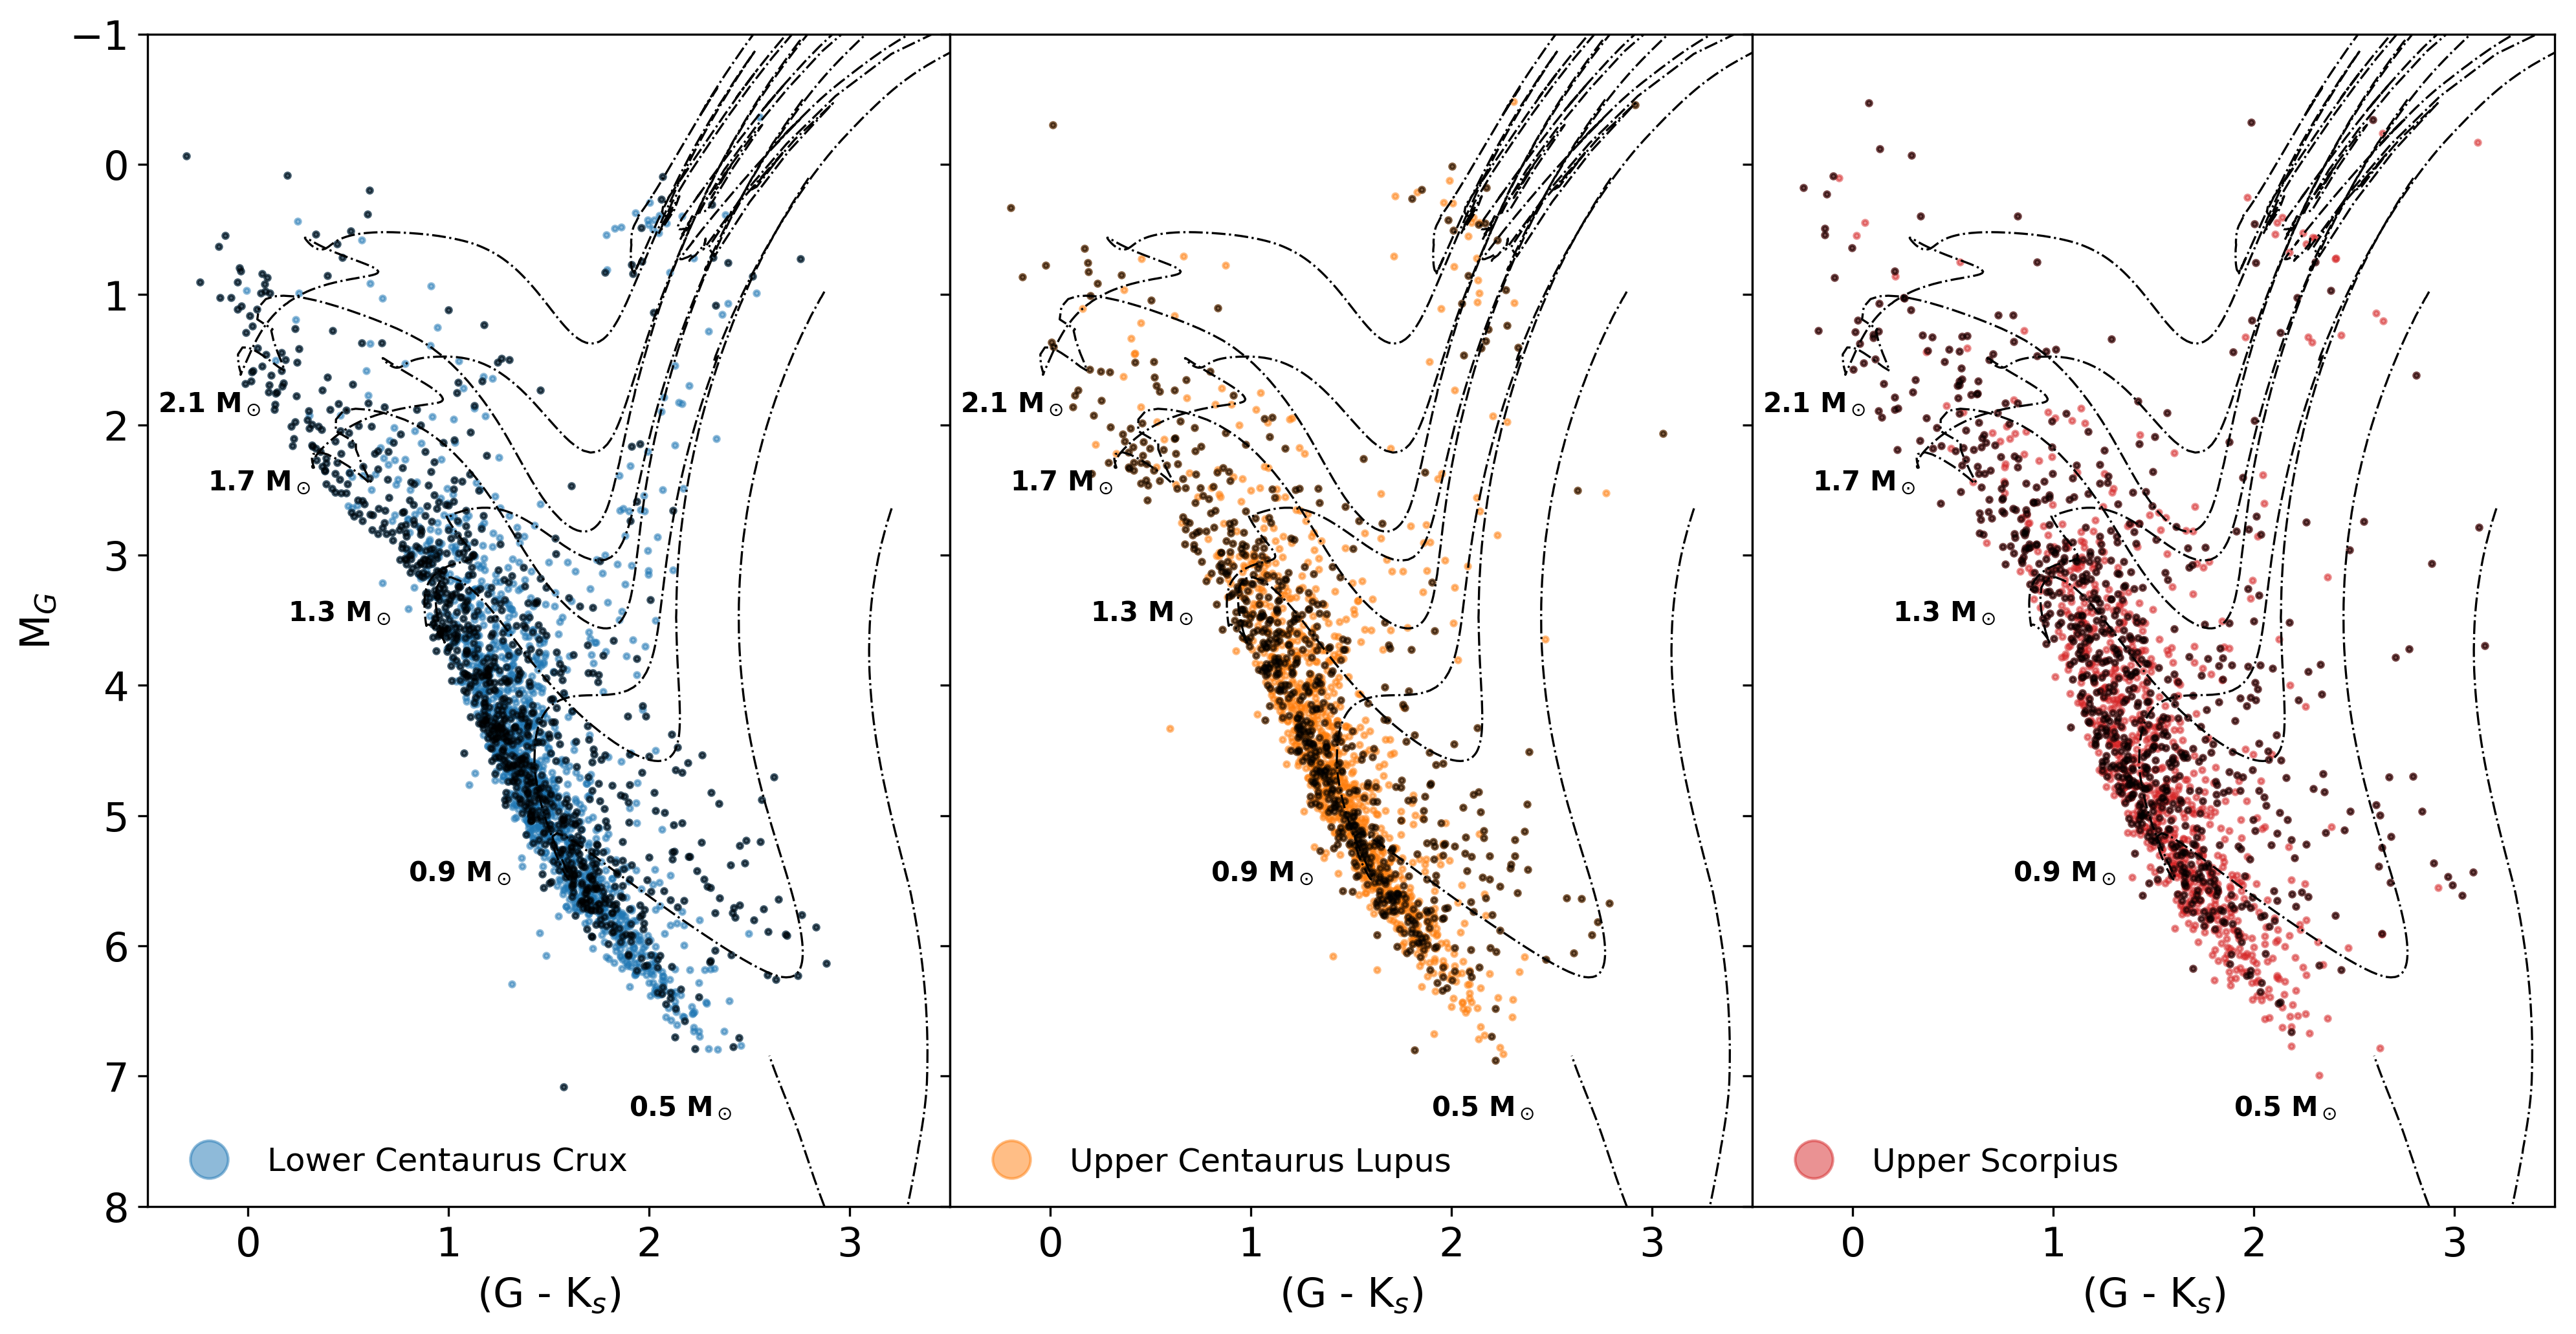
\includegraphics[width = 15cm, height = 8.5cm]{./Graficos/Capitulo_3/5_Sco-Cen/Mag_Col_diagram_4.png}} 
\caption{\scriptsize{Something!}}
\label{fig:Stellar_Tracks_1_appendix}
\end{figure}

\begin{figure}[!ht]
\centering
  \subfloat{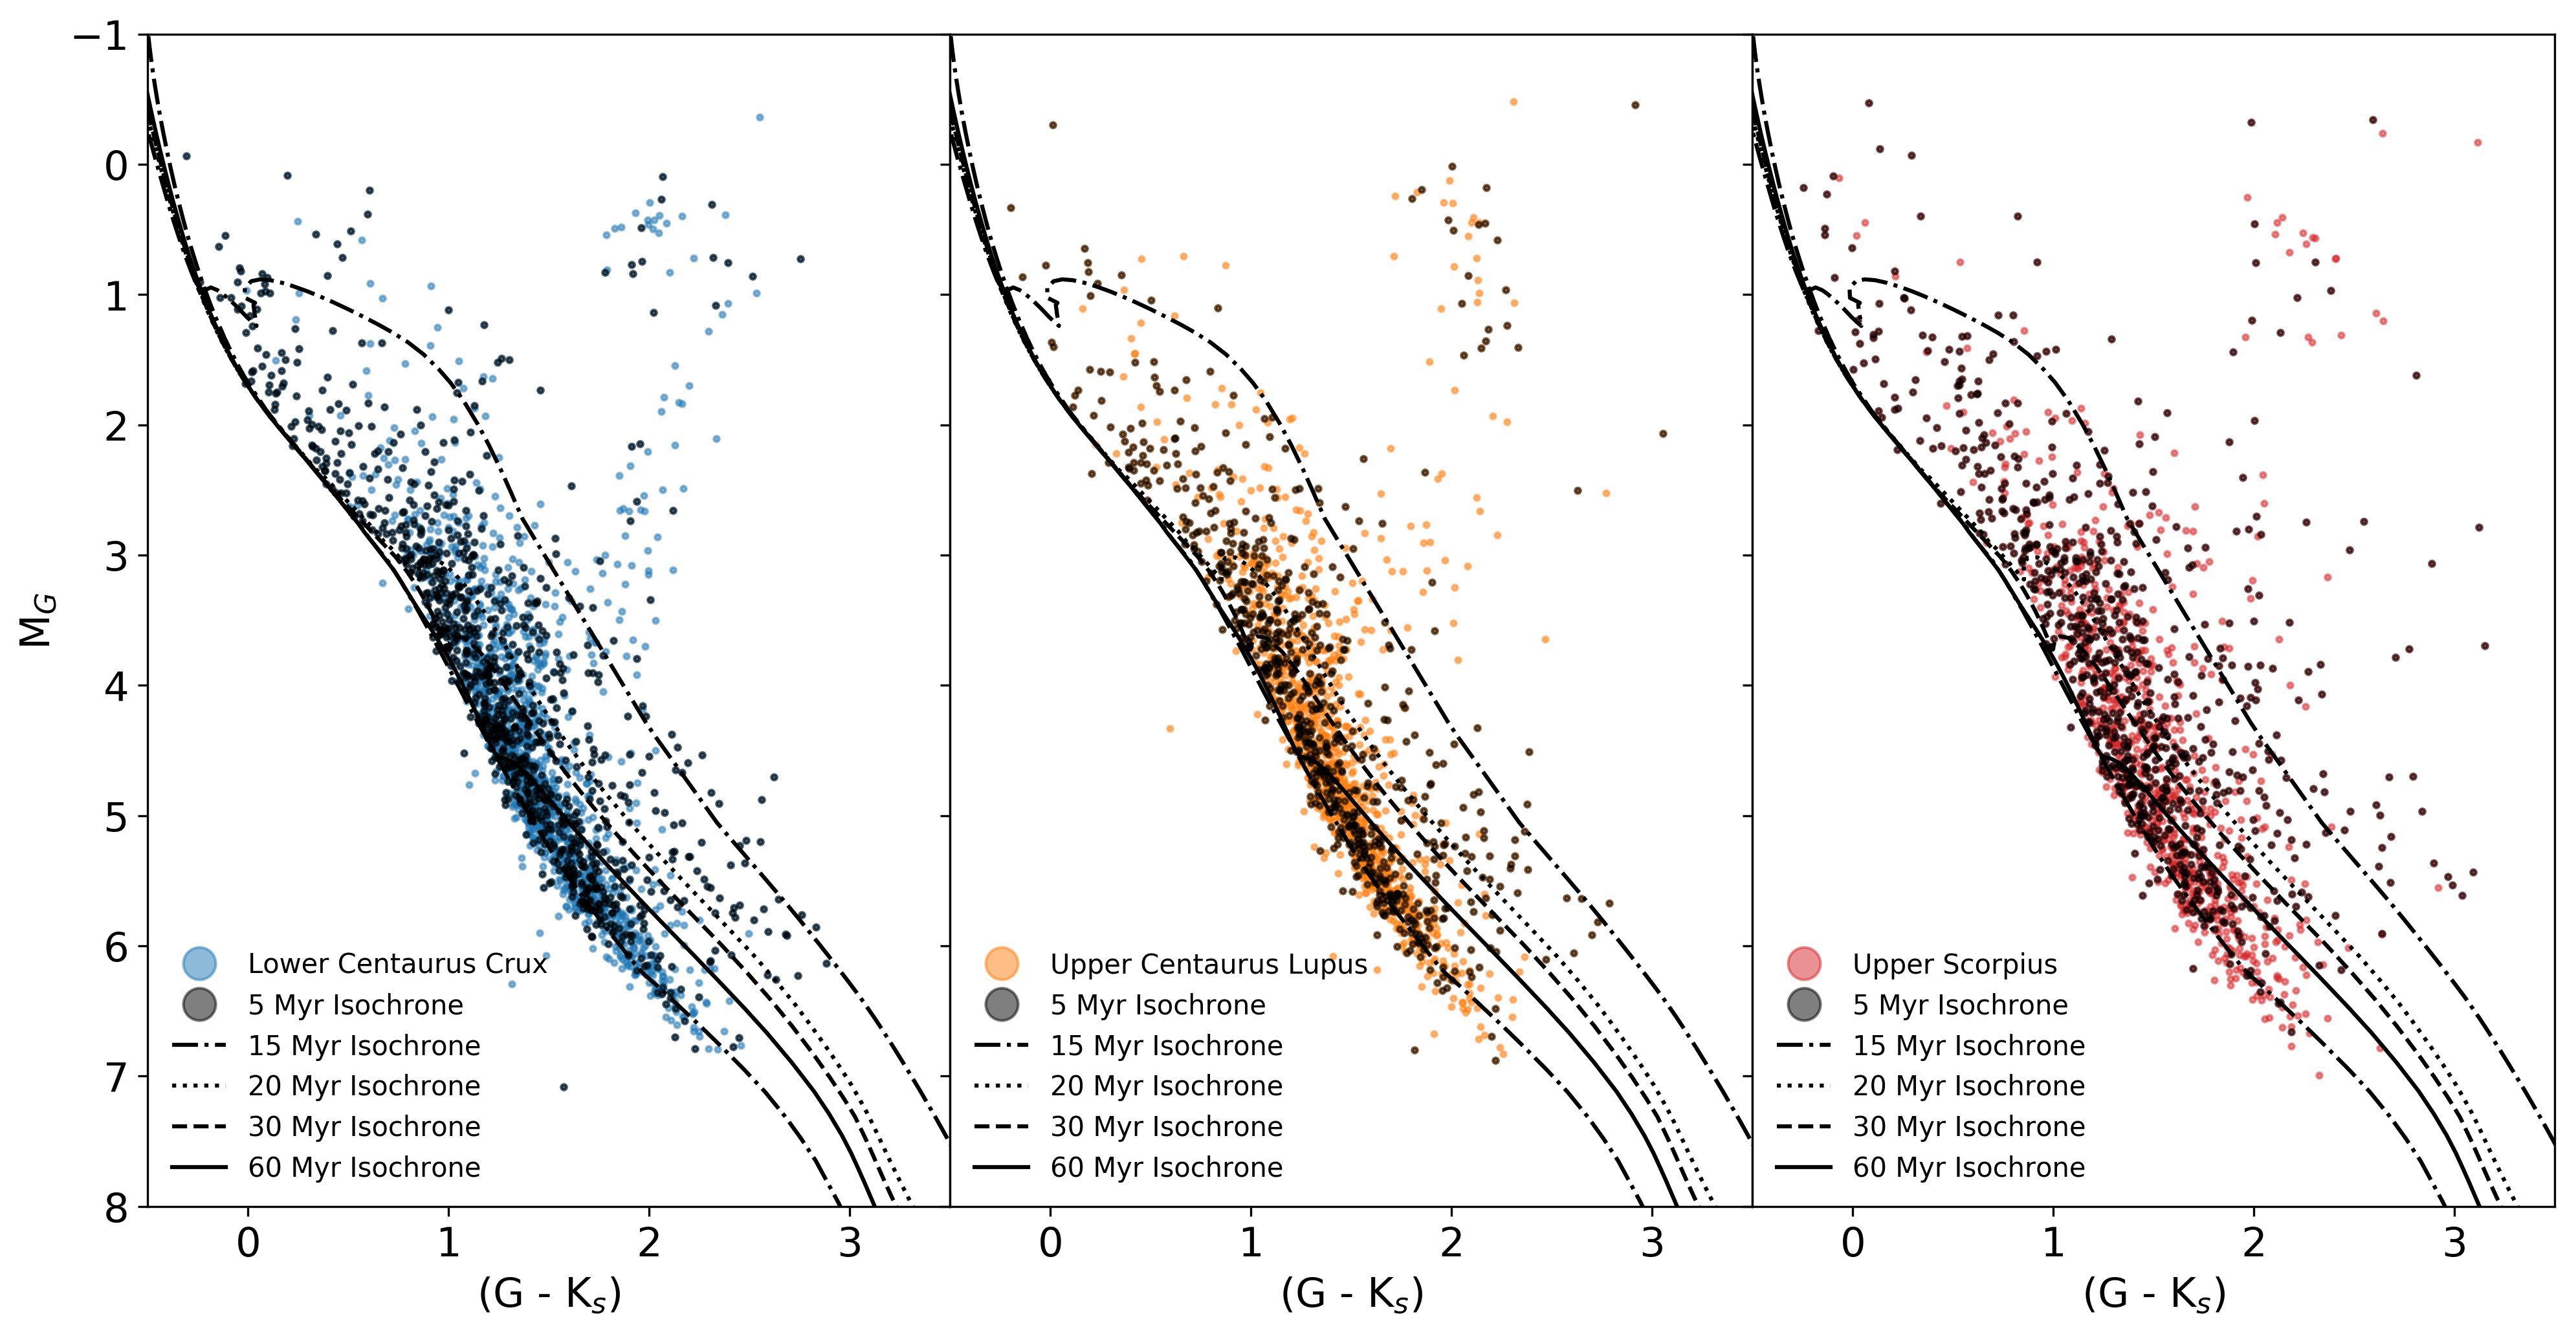
\includegraphics[width = 15cm, height = 8.5cm]{./Graficos/Capitulo_3/5_Sco-Cen/Mag_Col_diagram_3.png}} 
\caption{\scriptsize{Something!}}
\label{fig:Isochrones_1_appendix}
\end{figure}
